\documentclass{article}
\usepackage{amsmath,algorithm2e,caption,subcaption,url,fullpage,graphicx}

\title{CS 4641: Machine Learning\\
Project}
\date{December 3, 2019}
\author{Ethan MacGregor}

\begin{document}
\maketitle

\section{Dataset}

The dataset being used is a survey of men about masculinity and how they feel about certain aspects of it. It was used in a FiveThirtyEight article (\url{https://fivethirtyeight.com/features/what-do-men-think-it-means-to-be-a-man/}) and the raw data can be found in raw-responses.csv. (The questions corresponding to the answers in raw-responses.csv can be found in \url{https://github.com/fivethirtyeight/data/tree/master/masculinity-survey})\\

Our goal is to try to guess how masculine a respondent felt based on their other answers. The specific question is 'In general, how masculine or "manly" do you feel?' The men had five options: 'not at all masculine', 'not very masculine', 'somewhat masculine', 'very masculine' or no answer. We will try to guess this answer based on the respondent's other answers.\\

I chose this dataset because I thought it would be interesting if I was able to tease out real signal in this dataset. The metric that will be used to measure performance is the algorithms success rate in classifying testing data that it had never seen before.\\

\section{Algorithms}

We will be using three different classification algorithms and scoring them based on the accuracy of their classifications on testing data that they have never seen before.

\subsection{Random Forests}

Random forests are subclasses of decision trees. They work by examining their training data, selecting a subset of features randomly and then choosing the best of those features to split on based on its splitting criterion. The random forest will generate many trees (thus making a forest) and then classify a testing datapoint by returning the class that the most trees returned. This is called bagging.\\

Random forests perform better than decision trees in systems with greater max depth. This is because random forests limit overfitting through their random choice of features.\\

The hyperparameters we will test are:

\begin{itemize}
\item Number of estimators, meaning the number of trees in the random forest. In theory more estimators should always be good, but there comes a trade-off where more estimators has diminishing returns for the extra time spent. I tested 10, 100, 1000, and 5000 estimators.
\item The criterion to split on. The algorithm can choose to split on the result of the gini impurity or the information gain (entropy). Some datasets are better suited for one or the other, and our goal is to find out which is better for our dataset. I tested both.
\item Maximum depth. The default setting for this is unlimited max depth, and I expect this is where it will stay. Having a greater max depth can only limit run time and should likely only help classification performance. The values tested were 5, 10, 20, 50, and unlimited.
\end{itemize}

\subsection{Support Vector Machines}

A support vector machine is a method of transforming data that is not linearly separable into data that is through use of a kernel. For example, data that would be best fitted by a circular decision boundary is not linearly separable in that form, but it becomes linearly separable if transformed. SVM performs this transformation, linearly separates the data, and transforms back.\\

The hyperparameters tested were:

\begin{itemize}
\item The type of kernel. Of the non-linear kernels, we could use a polynomial kernel, an radial-based-focus kernel, and a sigmoid kernel. Some kernels are better for some datasets and our goal is to find out what kernel is best for our dataset.
\item Gamma, the kernel coefficient. A higher gamma will result in points far away from the decision boundary not being considered much, whereas a low gamma will mean the opposite. Our goal is to test which gamma produces the best results. Our tests are .001, .01, .1 and scale which is equal to $\frac{1}{n_features * X.var()}$ where X.var() is the variance of the dataset.
\end{itemize}

\subsection{Neural Networks}

Neural networks are logic circuits that mimic neuron structures inside the brain. Neural networks train on data and adjust their neuronal connections and logic based on what gets the best results. The rate of adjustment is called the learning rate and the way that neurons will fire based on their inputs is called the activation function. Neurons are structured in layers, with one input layer which takes the data, an output layer which returns the classification, and a number of hidden layers inside the network that make up most of the network. The structure and size of these layers can influence the performance of the network.\\

The hyperparameters tested were:

\begin{itemize}
\item Solver function. There are three possible solver functions, lbfgs, stochastic gradient descent, and adam.
\item Alpha. This is the learning rate. I tested .000001, .00001, .0001, .001, .01, and .1.
\item Activation function. This is the activation funtion that communicates information between neural network layers. This can be identity, which does nothing, logistic, which is the logistic sigmoid function, tanh, and relu, which is f(x) = max(0, x).
\item Maximum iterations. My expectation was that like estimators in the random forest, more is always better. This was tested with sgd, because  sgd performed best in the solver function and often got cut off by not having enough iterations, so it seemed appropriate to test it on sgd. The number of iterations tested were 100, 200, 500, and 1000.
\end{itemize}

One hyperparameter that was not tested was the shape of the neural network (I always used a (100, 75, 50) structure). This was not tested because the space for testing is much too large to represent in a couple of simple experiments.\\

\section{Hyperparameters}

For each hyperparameter tuned I have performed a number of experiments to try to reach an optimal setting. The experiments were conducted by training the algorithm on a training data set which comprised 25\% of the data, and then testing the algorithm on the remaining 75\% of the data. For each experiment, 20 trials were run and the results were recorded, including the mean, standard deviation, minimum, 25th percentile, median, 75th percentile, maximum, and the time it took to reach those results. The results are shown below and are each captioned with the hyperparameter being tuned and its value, along with the command-line command that can be used to reach the exact same figures.

\subsection{Random Forests}

The results are shown in figures 1-11. The best results for estimators were for 5000 estimators, but the gains over 1000 estimators were so small that it is not worth the enormous time increase. The best results for criterion was for gini, but the difference was very small and entropy also had a lower standard deviation, which could in some cases be more desirable. However, we will choose to use gini. As expected, an unlimited max depth produced better results for very little drop in time.\\

Results: 1000 estimators, gini, unlimited.

\begin{figure}
\begin{center}
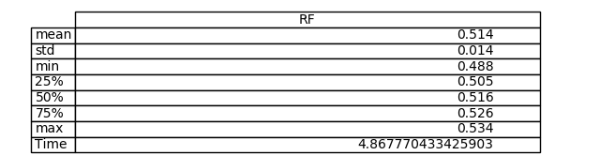
\includegraphics[width=8cm]{images/rf_10}
\caption{Random Forests (gini) with 10 estimators | python main.py -alg rf -estimators 10 -n 20 -seed 0}
\end{center}
\end{figure}
\begin{figure}
\begin{center}
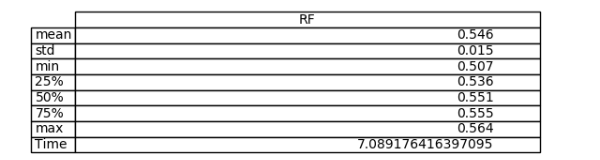
\includegraphics[width=8cm]{images/rf_100}
\caption{Random Forests (gini, unlimited) with 100 estimators | python main.py -alg rf -estimators 100 -n 20 -seed 0}
\end{center}
\end{figure}
\begin{figure}
\begin{center}
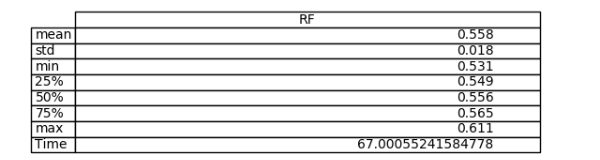
\includegraphics[width=8cm]{images/rf_1000}
\caption{Random Forests (gini, unlimited) with 1000 estimators | python main.py -alg rf -estimators 1000 -n 20 -seed 0}
\end{center}
\end{figure}
\begin{figure}
\begin{center}
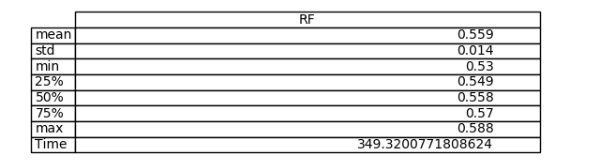
\includegraphics[width=8cm]{images/rf_5000}
\caption{Random Forests (gini, unlimited) with 5000 estimators | python main.py -alg rf -estimators 5000 -n 20 -seed 0}
\end{center}
\end{figure}
\begin{figure}
\begin{center}
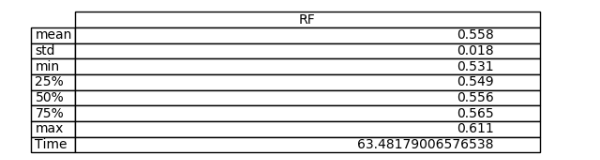
\includegraphics[width=8cm]{images/rf_gini}
\caption{Random Forests (1000 estimators, unlimited) with gini | python main.py -alg rf -criterion gini -n 20 -seed 0}
\end{center}
\end{figure}
\begin{figure}
\begin{center}
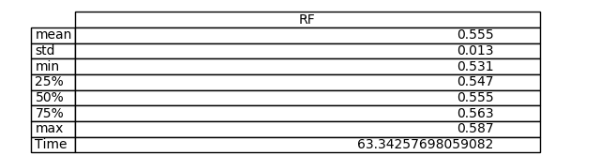
\includegraphics[width=8cm]{images/rf_entropy}
\caption{Random Forests (1000 estimators, unlimited) with entropy | python main.py -alg rf -criterion entropy -n 20 -seed 0}
\end{center}
\end{figure}
\begin{figure}
\begin{center}
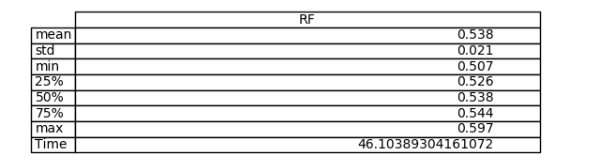
\includegraphics[width=8cm]{images/rf_d5}
\caption{Random Forests (gini, 1000 estimators) with max depth of 5 | python main.py -alg rf -depth 5 -n 20 -seed 0}
\end{center}
\end{figure}
\begin{figure}
\begin{center}
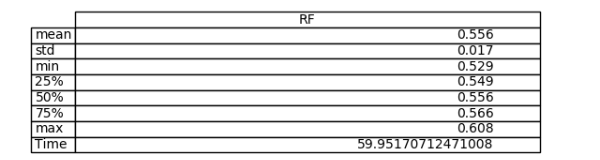
\includegraphics[width=8cm]{images/rf_d10}
\caption{Random Forests (gini, 1000 estimators) with max depth of 10 | python main.py -alg rf -depth 10 -n 20 -seed 0}
\end{center}
\end{figure}
\begin{figure}
\begin{center}
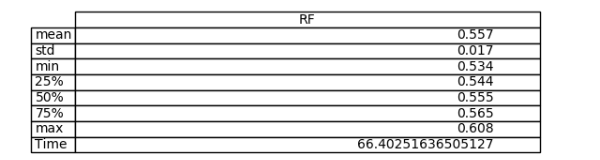
\includegraphics[width=8cm]{images/rf_d20}
\caption{Random Forests (gini, 1000 estimators) with max depth of 20 | python main.py -alg rf -depth 20 -n 20 -seed 0}
\end{center}
\end{figure}
\begin{figure}
\begin{center}
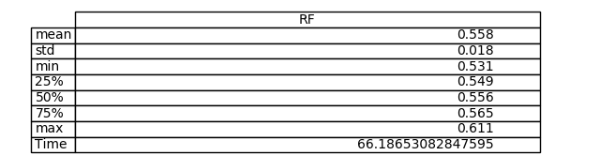
\includegraphics[width=8cm]{images/rf_d50}
\caption{Random Forests (gini, 1000 estimators) with max depth of 50 | python main.py -alg rf -depth 50 -n 20 -seed 0}
\end{center}
\end{figure}
\begin{figure}
\begin{center}
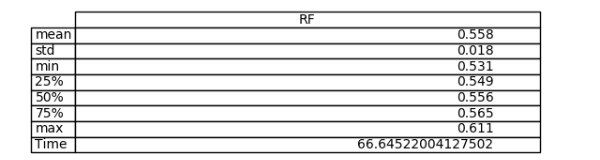
\includegraphics[width=8cm]{images/rf_dunlimited}
\caption{Random Forests (gini, 1000 estimators) with unlimited max depth | python main.py -alg rf -n 20 -seed 0}
\end{center}
\end{figure}

\subsection{Support Vector Machines}

The results are shown in figures 12-18. For gamma, scale very narrowly performed better than .01. The .1 and .001 gammas performed worse than scale and .01 in mean, but were also more consistent. In fact, the .1 and .001 gammas had almost identical results. My hypothesis is that for these large and small gammas, the algorithm decided that only picking 'somewhat masculine' in almost all cases was the best choice. We can see that these results are similar to what that method produces (shown in figure 35).\\

For the kernel the radial-based-focus kernel performed best, having the highest mean and only a very slightly larger standard deviation than the polynomial kernel.\\

Results: gamma: scale, kernel: rbf.

\begin{figure}
\begin{center}
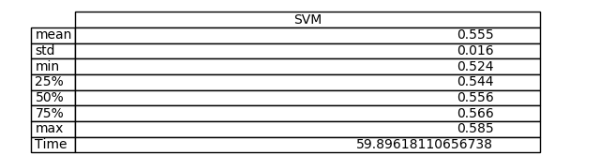
\includegraphics[width=8cm]{images/svm_poly}
\caption{Support Vector Machines (gamma='scale') with poly kernel | python main.py -alg svm -kernel poly -n 20 -seed 0}
\end{center}
\end{figure}
\begin{figure}
\begin{center}
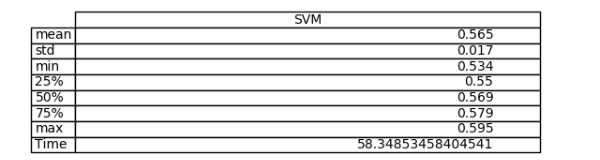
\includegraphics[width=8cm]{images/svm_rbf}
\caption{Support Vector Machines (gamma='scale') with rbf kernel | python main.py -alg svm -kernel rbf -n 20 -seed 0}
\end{center}
\end{figure}
\begin{figure}
\begin{center}
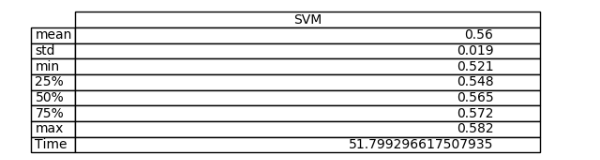
\includegraphics[width=8cm]{images/svm_sigmoid}
\caption{Support Vector Machines (gamma='scale') with sigmoid kernel | python main.py -alg svm -kernel sigmoid -n 20 -seed 0}
\end{center}
\end{figure}
\begin{figure}
\begin{center}
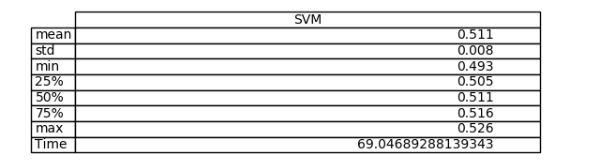
\includegraphics[width=8cm]{images/svm_1}
\caption{Support Vector Machines (kernel rbf) with .1 gamma | python main.py -alg svm -gamma .1 -n 20 -seed 0}
\end{center}
\end{figure}
\begin{figure}
\begin{center}
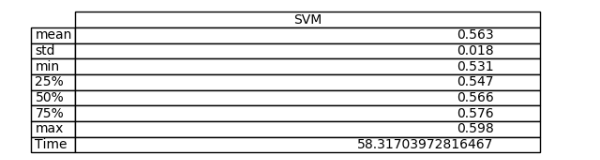
\includegraphics[width=8cm]{images/svm_01}
\caption{Support Vector Machines (kernel rbf) with .01 gamma | python main.py -alg svm -gamma .01 -n 20 -seed 0}
\end{center}
\end{figure}
\begin{figure}
\begin{center}
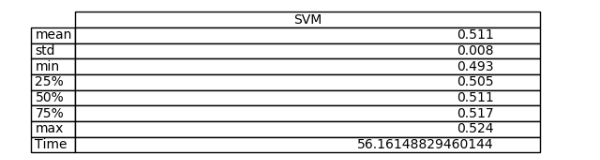
\includegraphics[width=8cm]{images/svm_001}
\caption{Support Vector Machines (kernel rbf) with .001 gamma | python main.py -alg svm -gamma .001 -n 20 -seed 0}
\end{center}
\end{figure}
\begin{figure}
\begin{center}
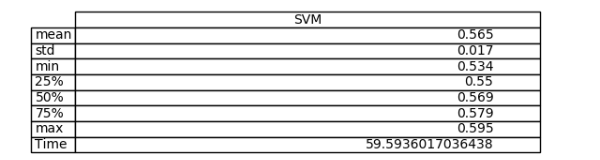
\includegraphics[width=8cm]{images/svm_scale}
\caption{Support Vector Machines (kernel rbf) with scale gamma | python main.py -alg svm -n 20 -seed 0}
\end{center}
\end{figure}

\subsection{Neural networks}

The results are shown in figures 19-35. The sgd solver performed significantly better than the other two methods despite the fact that it often got cut off before it converged. The best performing alpha was .01, although it took far more time than the other alphas. For activation functions, tanh outperformed logistic and identity, and very narrowly outperformed relu but not on a level that is significant, however, might as well pick the best one. Counter to my expectations, raising the max number of iterations did not improve the performance of the neural network, 200 max iterations produced far better results in far less time than 500 or 1000 max iterations. I think this may have been because of overfitting, the neural network got extremely good at predicting only the data in the dataset it was provided when it had extra time to do so, but this is only a guess.\\

Results: solver: sgd, alpha: .01, activation: tanh, iterations: 200

\begin{figure}
\begin{center}
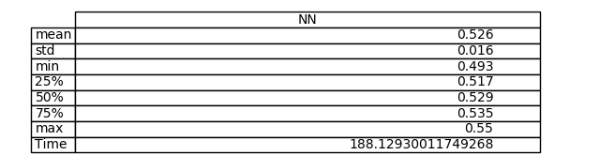
\includegraphics[width=8cm]{images/nn_adam}
\caption{Neural Network (relu, .0001, 200) with adam solver | python main.py -alg nn -solver -adam -n 20 -seed 0}
\end{center}
\end{figure}
\begin{figure}
\begin{center}
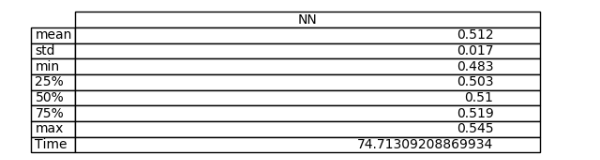
\includegraphics[width=8cm]{images/nn_lbfgs}
\caption{Neural Network (relu, .0001, 200) with lbfgs solver | python main.py -alg nn -solver lbfgs -n 20 -seed 0}
\end{center}
\end{figure}
\begin{figure}
\begin{center}
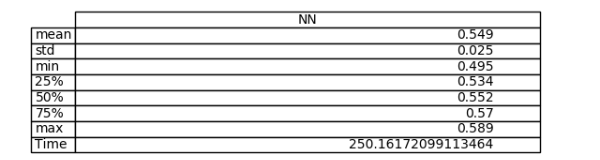
\includegraphics[width=8cm]{images/nn_sgd}
\caption{Neural Network (relu, .0001, 200) with sgd solver | python main.py -alg nn -solver sgd -n 20 -seed 0}
\end{center}
\end{figure}
\begin{figure}
\begin{center}
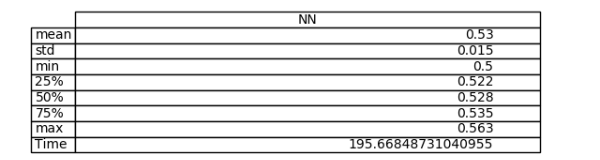
\includegraphics[width=8cm]{images/nn_000001}
\caption{Neural Network (adam, relu, 200) with alpha = .000001 | python main.py -alg nn -alpha .000001 -n 20 -seed 0}
\end{center}
\end{figure}
\begin{figure}
\begin{center}
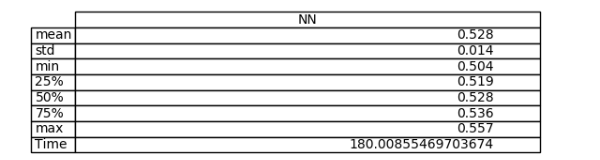
\includegraphics[width=8cm]{images/nn_00001}
\caption{Neural Network (adam, relu, 200) with alpha = .00001 | python main.py -alg nn -alpha .00001 -n 20 -seed 0}
\end{center}
\end{figure}
\begin{figure}
\begin{center}
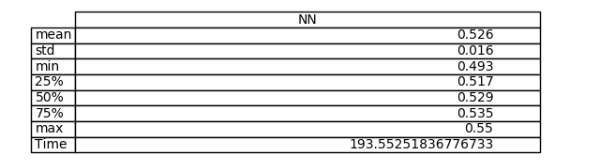
\includegraphics[width=8cm]{images/nn_0001}
\caption{Neural Network (adam, relu, 200) with alpha = .0001 | python main.py -alg nn -alpha .0001 -n 20 -seed 0}
\end{center}
\end{figure}
\begin{figure}
\begin{center}
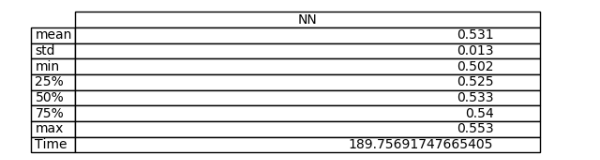
\includegraphics[width=8cm]{images/nn_001}
\caption{Neural Network (adam, relu, 200) with alpha = .001 | python main.py -alg nn -alpha .001 -n 20 -seed 0}
\end{center}
\end{figure}
\begin{figure}
\begin{center}
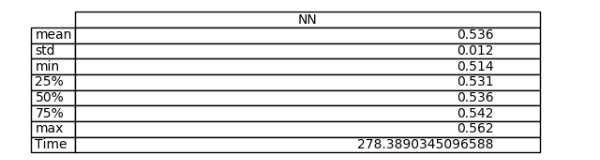
\includegraphics[width=8cm]{images/nn_01}
\caption{Neural Network (adam, relu, 200) with alpha = .01 | python main.py -alg nn -alpha .01 -n 20 -seed 0}
\end{center}
\end{figure}
\begin{figure}
\begin{center}
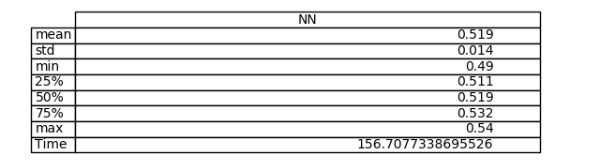
\includegraphics[width=8cm]{images/nn_identity}
\caption{Neural Network (adam, .0001, 200) with identity activation | python main.py -alg nn -activation identity -n 20 -seed 0}
\end{center}
\end{figure}
\begin{figure}
\begin{center}
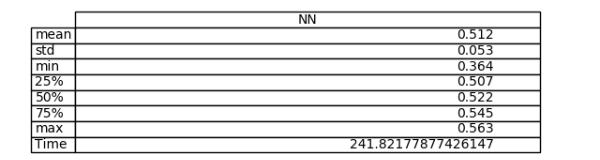
\includegraphics[width=8cm]{images/nn_logistic}
\caption{Neural Network (adam, .0001, 200) with logistic activation | python main.py -alg nn -activation logistic -n 20 -seed 0}
\end{center}
\end{figure}
\begin{figure}
\begin{center}
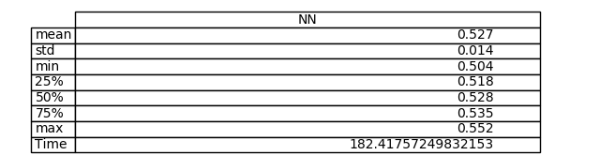
\includegraphics[width=8cm]{images/nn_tanh}
\caption{Neural Network (adam, .0001, 200) with tanh activation | python main.py -alg nn -activation tanh -n 20 -seed 0}
\end{center}
\end{figure}
\begin{figure}
\begin{center}
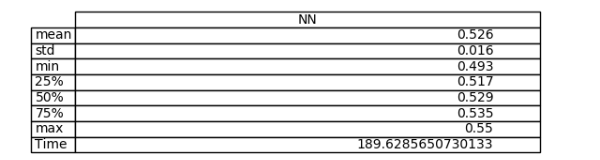
\includegraphics[width=8cm]{images/nn_relu}
\caption{Neural Network (adam, .0001, 200) with relu activation | python main.py -alg nn -activation relu -n 20 -seed 0}
\end{center}
\end{figure}
\begin{figure}
\begin{center}
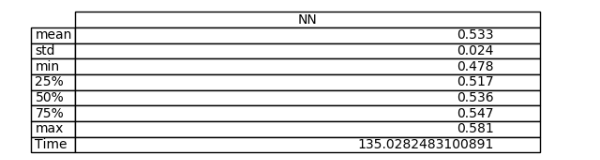
\includegraphics[width=8cm]{images/nn_100}
\caption{Neural Network (sgd, relu, .0001) with 100 iterations | python main.py -alg nn -solver sgd -iterations 100 -n 20 -seed 0}
\end{center}
\end{figure}
\begin{figure}
\begin{center}
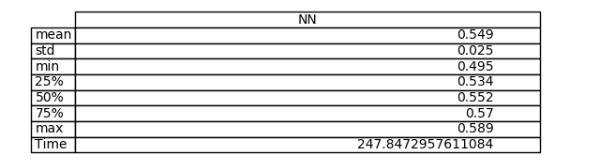
\includegraphics[width=8cm]{images/nn_200}
\caption{Neural Network (sgd, relu, .0001) with 200 iterations | python main.py -alg nn -solver sgd -iterations 200 -n 20 -seed 0}
\end{center}
\end{figure}
\begin{figure}
\begin{center}
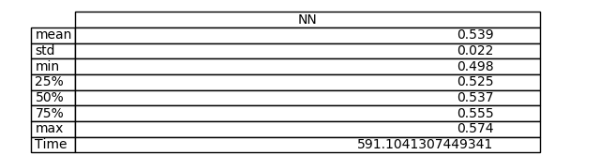
\includegraphics[width=8cm]{images/nn_500}
\caption{Neural Network (sgd, relu, .0001) with 500 iterations | python main.py -alg nn -solver sgd -iterations 500 -n 20 -seed 0}
\end{center}
\end{figure}
\begin{figure}
\begin{center}
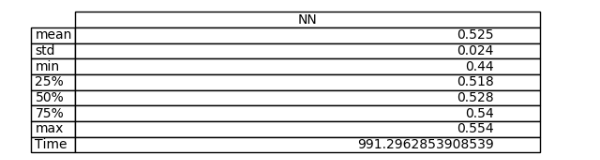
\includegraphics[width=8cm]{images/nn_1000}
\caption{Neural Network (sgd, relu, .0001) with 1000 iterations | python main.py -alg nn -solver sgd -iterations 1000 -n 20 -seed 0}
\end{center}
\end{figure}

\section{Algorithm performance}

Figures 35 and 36 are a table and a graph respectively comparing the three algorithms performance across 50 trials, along with a fourth algorithm I have added. This algorithm simply guesses that each man sees himself as 'somewhat masculine.' 'Somewhat masculine' was the most common response among the surveys, so I added this as a control algorithm to judge whether the algorithms were actually finding real signal in the dataset.\\

The experiment was conducted by training the algorithms on a training data set which comprised 25\% of the data, and then testing the algorithms on the remaining 75\% of the data. Each trial the algorithms trained and tested on the exact same data to ensure fairness.\\

All algorithms are using the optimal hyperparameters determined in the previous section.\\

\begin{figure}
\begin{center}
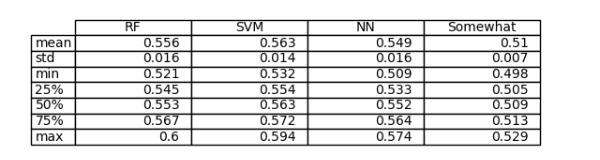
\includegraphics[width=8cm]{images/all_alg_table}
\caption{All algorithms (with optimal hyperparameters) compared in a table | python main.py -alg all -n 50 -seed 0}
\end{center}
\end{figure}
\begin{figure}
\begin{center}
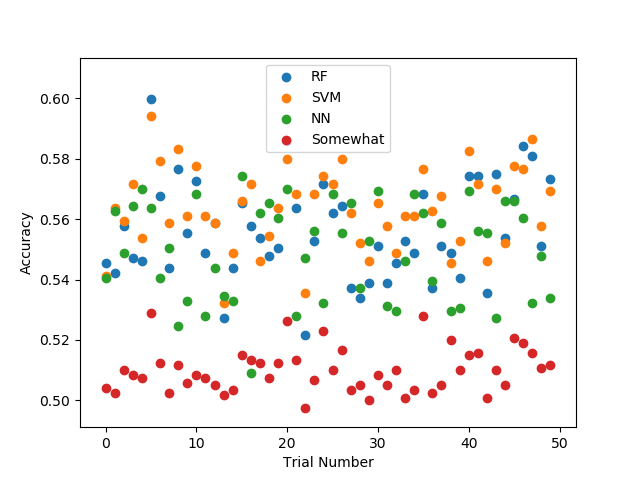
\includegraphics[width=8cm]{images/all_alg_graph}
\caption{All algorithms (with optimal hyperparameters) compared in a graph | python main.py -alg all -n 50 -seed 0}
\end{center}
\end{figure}

Based on the means calculated, the support vector machine algorithm performed the best, followed by the random forests, and then the neural network. All outperformed the control algorithm. The standard deviation shows that SVM was most consistent but all were fairly consistent. The random forest reached the highest maximum score and the neural network the lowest.

\section{Conclusion}

Through testing machine learning algorithms on this dataset, we can see there was real signal that allowed us to make informed guesses on the importance of masculinity to the respondents. This is shown by the fact that the algorithms were consistently able to outperform the control algorithm. \\

The support vector machine algorithm performed the best, followed by the random forests, and then the neural network. \\

The neural network had some low lows, we can see that there in trial \#16 the neural network actually underperformed the control algorithm. The disappointing performance of the neural network may be due to its shape; perhaps a different shape may have helped it perform better. This was not tested because the experiment space was too large, but perhaps someone with more machine learning expertise may have been able to pick a neural network shape that would have performed very well on this dataset.\\

There seemed to be a hard cap on the accuracy of the algorithms, as the max any of the algorithms every achieved was 60\% accuracy. This indicates that while the signal existed in the data, it may have been weak, or there may have been too much noise drowning it out. \\

All this said, I would choose the support vector machine model if I was to work on similar real-world data. It had the best mean performance and the lowest variance, few hyperparameters to tune, and worked similarly quickly to the random forest model and much faster than the neural network. SVM's 25th percentile outcome was better than the 50th percentile outcome of RF and NN, which really underscores its optimality and consistency.

\section{Acknowledgments}

I made heavy use of the scikitlearn libraries to run the algorithms and the documentation to help me understand what it was actually doing. \\

I used the pandas python library for easy data transfer and manipulation which let me use one-hot encoding to allow the algorithms to properly understand non-numerical data.\\

I used the following tutorial to initially understand how to manipulate my data and one-hot encode it: \url{https://towardsdatascience.com/random-forest-in-python-24d0893d51c0}\\

Thanks of course to FiveThirtyEight for providing the data which can be found at \url{https://github.com/fivethirtyeight/data/tree/master/masculinity-survey}

\end{document}